\chapter{Combinatioria}
\section{Árbol de combinación}
A continuación, se muestra un ejemplo de árbol de combinación que utiliza la técnica
\textit{Base Choice} para el cálculo de las combinaciones posibles de un sistema de
tres variables de entrada, en este caso $BI$, $R$ y $n_{E}$.

\begin{minipage}{\linewidth}
	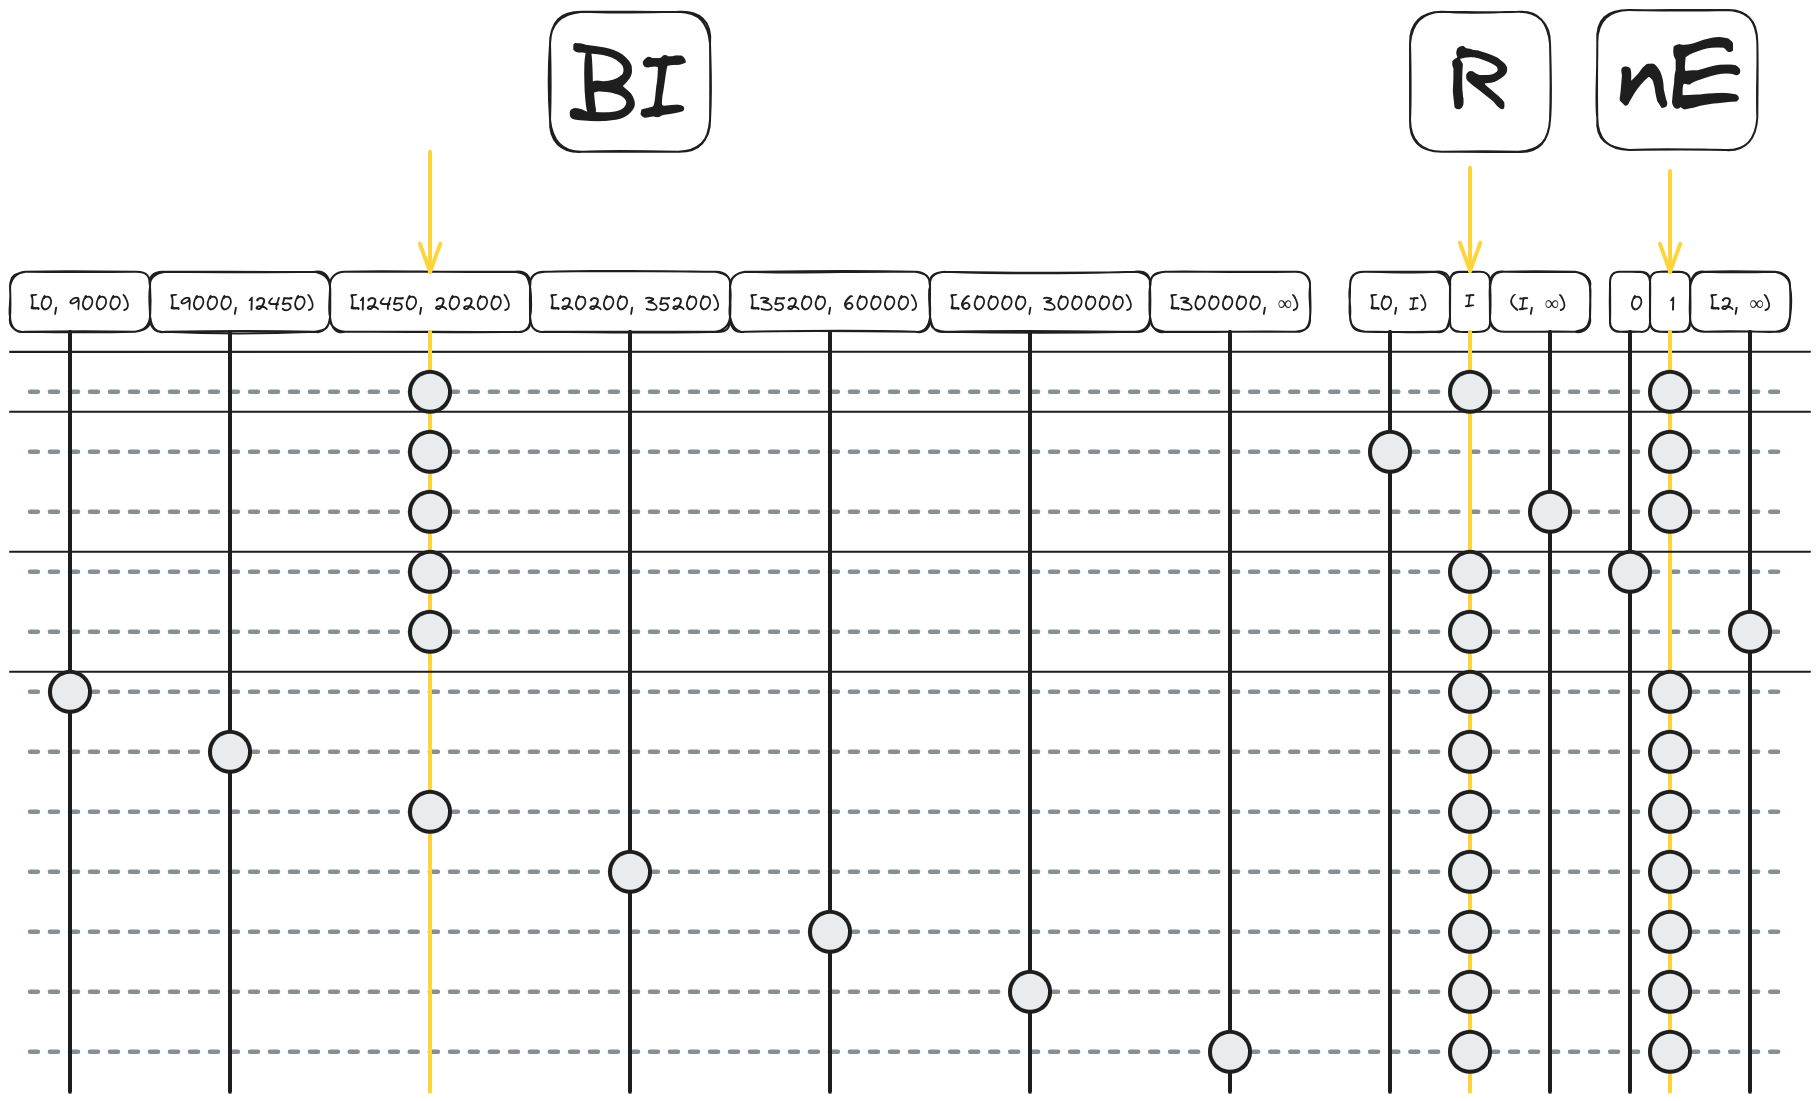
\includegraphics[width=\textwidth]{arbol.png}
	\captionof{figure}{Árbol de decisiones \textit{base choice} con tres variables}
\end{minipage}

En el diagrama anterior, se resaltan los casos seleccionados como ``base'' en amarillo.

\section{Ejemplo de caso de prueba}
A continuación, se muestra un ejemplo de caso de prueba del árbol anterior (último caso
de la variación de la variable $n_{E}$).
\begin{table}[H]
	\centering
	\captionof{figure}{Ejemplo de caso de prueba de combinación}
	\begin{tabular}{l|c c c|r r r}
		\hline
		\multirow{2}*{\bf{ID}} & \multicolumn{3}{c|}{\textbf{Entradas}} & \multicolumn{3}{c}{\bf{Salidas}} \\
		\cline{2-7}
		& $BI$ & $R$ & $n_{E}$ & Obligatoriedad & Máx. grav. & Resultado \\
		\hline
		\hline
		CP99 & 20000€ & $I$€ & 3 & Sí & 24\% & Sin cambios \\
		\hline
	\end{tabular}
\end{table}
